\section{Projektstruktur}
\label{sec:projektstruktur}
Dieses Kapitel soll eine \"Ubersicht liefern, wie die einzelnen Komponenten des Projekts interagieren. Das Software-Framework Robot Operating System\cite{ROS} (kurz ROS) stellt dabei f\"ur die einzelnen Funktionalit\"aten die Kommunikation zur Verf\"ugung. \\\\
\begin{figure}[h]
	\centering
	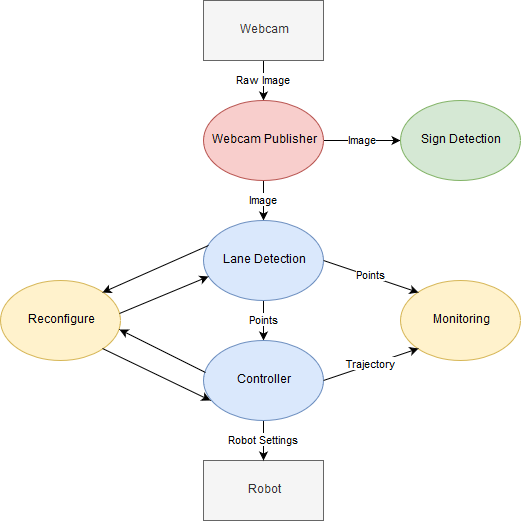
\includegraphics[width = 0.8\textwidth]{images/Projektaufbau.png}
	\caption{\"Ubersicht der einzelnen Komponenten des Projekts}
	\label{fig:projektaufbau}
\end{figure}
%TODO: der Controller heißt eigentlich trajectory_planning... Ist das bewusst so benannt? (Frederic)
\\
Abbildung \ref{fig:projektaufbau} zeigt die schematische Projektstruktur graphisch auf und erkl\"art sich folgenderma\ss{}en:
\begin{itemize}
\item Der \textbf{\textit{Webcam Publisher}} empf\"angt das rohe Kamerabild der \textbf{\textit{Webcam}} und nimmt Voreinstellungen, wie die Aufl\"osung vor. Dieses Bild wird an die Komponenten \textbf{\textit{Sign Detection}} und \textbf{\textit{Lane Detection}} verteilt.
\item Die \textbf{\textit{Lane Detection}} verarbeitet das Bild, ermittelt daraus Punkte der Fahrbahnmarkierungen und sendet diese dann an den \textbf{\textit{Controller}} weiter.
\item Mithilfe der Punkte wird durch den \textbf{\textit{Controller}} eine Trajektorie ermittelt und Motor- und Lenkeinstellungen berechnet, welche an das Roboterauto zur\"uckgegeben werden.
%TODO: Roboterauto richtiger Begriff? (Frederic)
\item Das \textbf{\textit{Monitoring}} nimmt die Ergebnisse der \textbf{\textit{Lane Detection}} und des \textbf{\textit{Controller}} und stellt diese graphisch zu \"Uberpr\"ufungszwecken dar.
\item \textbf{\textit{Reconfigure}} stellt dabei mehrere Werte sowohl der \textbf{\textit{Lane Detection}} als auch des \textbf{\textit{Controller}} w\"ahrend des Betriebs des Roboterautos, ein.
\end{itemize}